\chapter{GPU Based Algorithms for Spectrum Sensing in Cognitive Radio Networks}

\section{Introduction}


\section{Related Work}
Discuss work done with general spectrum sensing.
Discuss early work of FAM implementation in Matlab.
Discuss work done on performing the FAM algorithm on the cell processor.
Discuss lack of previous work on porting cognitive networking algorithms onto the GPU architecture.


\section{Spectrum Sensing Algorithms}
The cognitive networking model assumes two kinds of users, primary and secondary users.  Primary users are those who have privileged rights to a licensed spectrum for their commercial or public usage.  Secondary users are those users who do not have privileged rights but still have access to licensed spectrums.  These secondary users must opportunistically use unallocated spectrum resources when they are available, but vacate those resources when a primary user desires access to them.  In order to facilitate the intelligent usage of unallocated resources, secondary users must have a means of detecting the unused portions of a spectrum.  Spectrum sensing algorithms are designed to quickly and accurately detect the unoccupied spectrum segments available for use by secondary users.

There are several methods available to perform this kind of detection.  Each method is suited to different types of environments and signal types.  We have chosen to target two methods for this paper, energy detection and cyclostationary spectral analysis.

\subsection{Energy Detection}
\label{sect:energy_detect}
One method available to perform spectrum sensing is through the use of energy detection methods.

\subsection{Cyclostationary Spectral Analysis}
\label{sect:cyclo}
Another method of performing spectrum sensing is through the use of cyclostationary spectral analysis.  This method is typically chosen to detect low SNR modulated signals because of its ability to distinguish between modulated signals, interference, and noise in low signal to noise ratios \cite{FenChenWan08}.  Cyclic spectral analysis algorithms work by estimating the correlation between spectral components of signals.  Spectral components are the complex envelopes of narrowband, bandpass components of a signal \cite{RobBroLoo91}.  This correlation is described by the spectral correlation density (SCD) function.  This function describes the localization in the frequency domain of the amount of time-correlation between frequency-shifted versions of a given signal $x(t)$ \cite{Costa96}.  The SCD is represented by the two dimensional cyclic frequency and signal frequency space \cite{FenChenWan08} called the bifrequency plane.  Presence of a signal can then be detected through the use of the SCD function \cite{Costa96}.

For our work we have chosen to implement the well known FFT Accumulation Method (FAM) to estimate the SCD function.  The FAM algorithms is of specific interest for adaptation onto a GPU because it is able to take great advantage of data-parallelism.  The following section gives details about the FAM algorithm

\subsubsection{FFT Accumulation Method}
\label{sect:FAM}
The FFT Accumulation Method works by dividing the bifrequency plane into smaller regions called channel pair regions and computes the estimates one block at a time using FFT's \cite{Pace03}.  The values of the SCD function are described by equation \ref{eq:SCD}.

\begin{equation}
S^{\alpha}_{X_{N^\prime}} {(n L, f)}_{\Delta t} = \sum_{r=0}^{P-1} X_{N^\prime}(r L,f + \frac{\alpha}{2}) X_{N^\prime}^*(r L, f - \frac{\alpha}{2})
\label{eq:SCD}
\end{equation}

Equation \ref{eq:ComplexDemod} describes the computation of the channel pair regions, also called the complex demodulates.

\begin{equation}
X_{N^\prime}(n,f) = \sum_{n=0}^{N^\prime - 1} w(n) x(n) e^{-(i 2 \pi f n)/N^\prime}
\label{eq:ComplexDemod}
\end{equation}

Here \begin{math}w(n)\end{math} is a data tapering window (e.g., Hamming window), L is a decimation factor in the frequency domain \cite{FenChenWan08}, P is equal to \begin{math}N / L \end{math} where $N$ is the total number of samples in the signal and $N^\prime$ is equal to the number of samples in each complex demodulate.  In choosing the value of \begin{math}N^\prime \end{math} we must consider that the time-frequency resolution product \begin{math}N/N^\prime\end{math} must satisfy the condition \begin{math}N/N^\prime >> 1\end{math} in order to have a statistically reliable measurement \cite{RobBroLoo91}.  The value of $L$ is typically chosen to be \begin{math}L \le N^\prime / 4\end{math} in order to provide a good compromise between computational efficiency and minimizing cycle leakage and aliasing \cite{RobBroLoo91}.

The algorithm then occurs in three steps.  First the channelization is performed by an $N^\prime$-point FFT being hopped over the signal data in blocks of $L$ samples.  The results from the FFT are then frequency shifted to baseband.  This produces the decimated complex demodulates \cite{RobBroLoo91}.  Second the product sequences are computed.  These are computed by multiplying each complex demodulate by the complex conjugate of each of the others \cite{Costa96}.  Once these are computed a $P$-point FFT is applied.

%Maybe break this section off into a section below on the GPU's applicability to cognitive networking.
The parallelism of this algorithm is a direct result of the independence of the product sequences both before and after their computation \cite{RobBroLoo91}.  This means that at each step of the algorithm, we can take advantage of high degrees of data-parallelism.  In step one, each complex demodulate can be independently computed.  The same can be said of computing the product sequences of step 2 and during step three the $P$-point FFT's can be applied independently to each of the product sequences.  This very high level of data-parallelism combined with the high level of computation makes this algorithm a strong candidate for GPU based processing.


\section{Why Use the GPU?}
The GPU is a highly parallelized, multi-threaded, multi-cored processor.  The GPU is well suited to address problems that can be expressed as data-parallel computations - the same program executing on many data elements in parallel - with high arithmetic intensity \cite{Nvidia08}.  A single GPU is capable of computing thousands of threads simultaneously with incredibly optimized performance for high precision floating point operations.  Figure \ref{fig:cpu_vs_gpu_arch} illustrates the difference in architecture between CPUs and GPUs.  Since GPUs are specialized for data parallelism, they have a lower requirement for flow control and memory access latency can be hidden with high intensity calculations instead of data caches \cite{Nvidia08}.

%should use some of the diagrams from the Nvidia CUDA Programming Guide
\begin{figure*}[htp]
\begin{center}
 \scalebox
 {0.80} % h_length
 {
 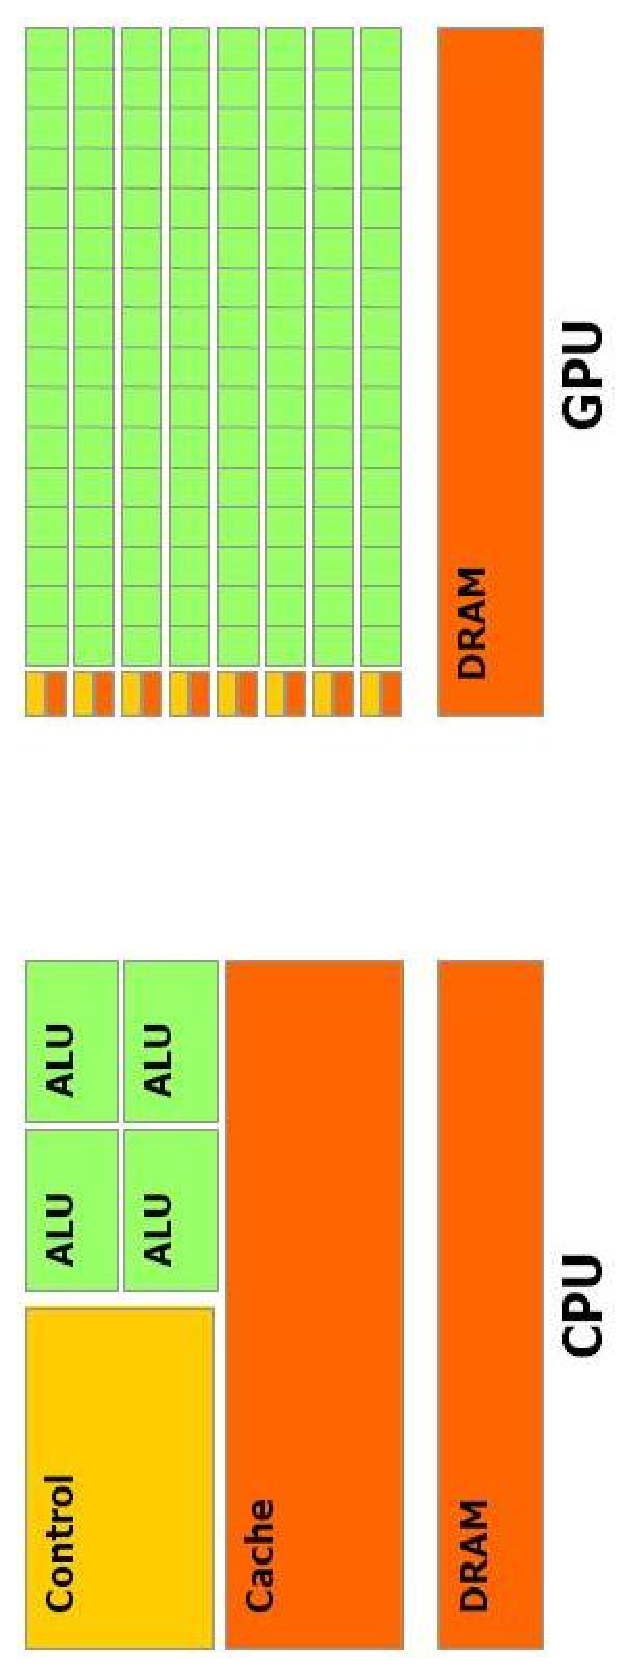
\includegraphics[angle=270,scale=0.5]{images/gpu_images/cpu_vs_gpu_arch.eps}
 }
\end{center}
\caption{\label{fig:cpu_vs_gpu_arch}
Basic diagrams comparing the differences in the architectures between a CPU and a GPU.  The GPU clearly devotes more transistors to data processing \cite{Nvidia08}.
}
\end{figure*}

%Not sure this fits in this section or maybe just this location, see if it can be moved or needs to be removed.
Through NVIDIA's CUDA computing engine, the massively parallel structure of GPU's can be harnessed for general purpose computing.  CUDA provides extensions to industry standard languages, such as C and Python, to access the parallel computing capabilities of NVIDIA based GPU's.  CUDA provides a set of three key abstractions - a hierarchy of thread groups, shared memory, and barrier synchronization - that are exposed to the programmer through these language extensions \cite{Nvidia08}.

\subsection{Application to Cognitive Networking}
Cognitive networking algorithms rely on extremely fast computations of large sets of complex data in order to provide the necessary real time requirements for performance.  In many cases, these computations can take advantage of parallel computing architectures, such as those offered by GPUs, to help increase their performance.

One of the primary operations relied upon by many of the cognitive networking algorithms is the computation of Fast Fourier Transforms.  This is a common operation in many signal processing algorithms and is one that can benefit from high degrees of parallelism.  Table \ref{tbl:matlab_vs_gpu_fft} shows a comparison of computation times for FFT's of various size using Matlab and using CUDA.  It is clear that CUDA is able to perform this operation much faster than  Matlab as the size of the FFT increases.  Algorithms such as the FFT Accumulation Method (\ref{sect:FAM}) make heavy use of this operation so a fast implementation can make a big difference in the algorithms overall performance.

%need to get the matlab vs gpu fft timings from Boris
\begin{table*}
\begin{center}
\begin{tabular}{|l|l|l|l|l|}
\hline
 & \multicolumn{2}{|c|}{Citation Graph} & \multicolumn{2}{|c|}{Inet4500} \\
\hline
Metric & Weight Range & Ratio & Weight Range & Ratio \\
\hline
1-Ring& 1 to 75 & 0.0721 & 1 to 942 & 0.2093 \\
2-Ring & 2 to 380 & 0.3687 & 2 to 3585 & 0.79667 \\
3-Ring & 3 to 763 & 0.7414  & 3 to 4432 & 0.9842 \\
Shortest Path & 0 to 85284 & 83.2039 & 0 to 12926842 & 2872.6315 \\
Dist to Leaf & 0 to 7 & 0.0068 & 0 to 4 & 0.0008 \\
Dist to Center & 1 to 10 & 0.0087 & 1 to 6 & 0.0011 \\
Eccentricity & 9 to 17 & 0.0087 & 5 to 9 & 0.0008 \\
\hline
\end{tabular}
\caption{This table lists the Weight Range to \# of Nodes ratios for each metric and each graph they were run against.}
\label{tbl:matlab_vs_gpu_fft}
\end{center}
\end{table*}

\subsection{Availability and Cost Effectiveness}
The GPU is also a very cost effective and readily available solution.  Almost every desktop, and even some laptop computers, sold today have some version of a GPU residing in them.  Even those desktop computers without a GPU can add them in easily and at a fairly reasonable price.  Although cell processors are also very powerful and highly parallelizable, they are not yet as widely available as GPU's in everyday computing devices.  The only commercially available device with a cell processor is the Sony Playstation 3.  It is possible to use the cell processor in the Playstation 3 for general purpose computing, but it requires the purchase of and presence of the entire Playstation 3 hardware setup.  From both a cost and availability standpoint, GPU's are an excellent choice for adapting cognitive networking algorithms.


\section{Experimental Setup}
text about how we tested these algorithms

\subsection{Test Platform}
details about the computer used for execution.

\subsection{Test Data}
details about the data sets we used for testing these algorithms



\section{Results}
section outlining our experimental findings

\subsection{Energy Detection}
\label{sect:energy_detect_result}
section specifically for our results relating to the performance of the energy detection method.  Include timings of calculations on matlab implementation and on the gpu.  compare generated results between both versions.  possibly compare these results against those found in other papers.

\subsection{FFT Accumulation Method}
\label{sect:FAM_result}
section specifically for our results relating to the performance of the FAM method.  Include timings of calculations on matlab implementation and on the gpu.  compare generated results between both versions.  possibly compare these results against those found in other papers.

\section{Conclusion}
a brief conclusion about our work on this topic.
